\section{Introduction}
\label{sec:introduction}
Process mining uses timestamped event records to study operational processes~\cite{vanDerAalst2016processmining}. Many manual factory tasks leave no such records. An information system may record an order or machine checkpoint while missing how a worker loads parts, moves material, checks a component, or switches tools. Video can make some of this work observable, but it does not directly provide the case identifiers, labels, and event boundaries that process mining needs~\cite{kratsch2022video}.

Egocentric video records work from the camera wearer's perspective. The public Egocentric-10K resource provides factory recordings of this kind~\cite{build2025egocentric}. Figure~\ref{fig:egocentric} illustrates the viewpoint. Turning recordings into event logs requires decisions about what constitutes an event, which names to use, and how to interpret time. These are measurement decisions as well as extraction tasks. A well-formed log can still misrepresent the work if a behavior is omitted, a boundary is estimated poorly, or an analytical category hides a recorded action.

\begin{figure}[htbp]
\centering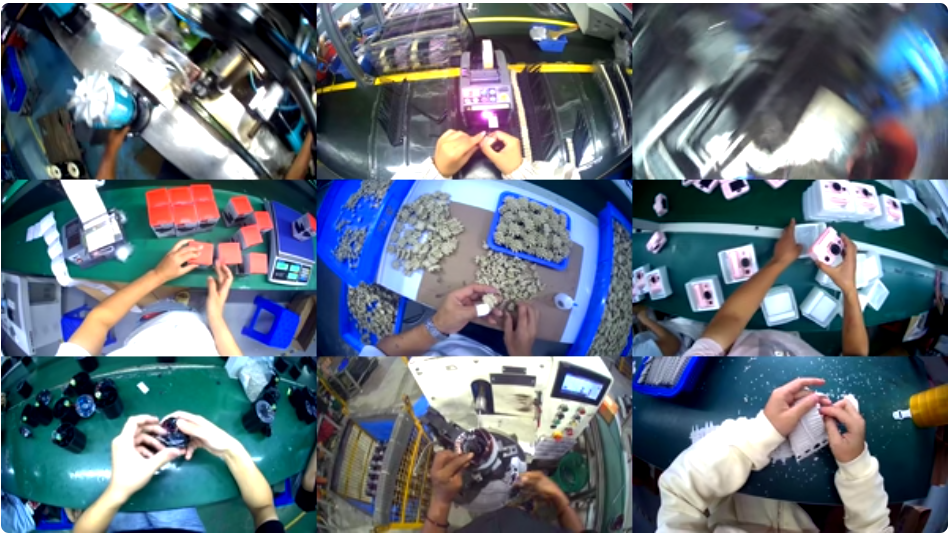
\includegraphics[width=0.85\linewidth]{figures/egocentric10k.png}
\caption{Example frames from Build AI's Egocentric-10K resource~\cite{build2025egocentric}. They illustrate the camera viewpoint, rather than the accuracy of the derived event labels.}
\label{fig:egocentric}
\end{figure}

Video-to-log construction already includes language-model-based methods. Vid2log uses a pretrained vision-language model to interpret video and construct event data~\cite{gavric2024multimodal}. First-person workflow extraction also predates this study~\cite{petersen2013workflows,pham2018workflow}. The question here is how to build a shared event representation from the available factory recordings and explain its consequences for process analysis. In particular, naming an activity, assigning an episode to that name, and mapping the label into a measurement category are separate decisions. A shared vocabulary makes within-factory comparison possible, but does not by itself make the resulting measurements accurate or comparable across tasks.

We study a five-stage pipeline that produces timestamped transcripts, worker summaries, factory reports and vocabularies, per-video events, and merged logs. It induces a vocabulary across the recorded workers in each factory before assigning event labels from their transcripts. Its application covers six factories, 59 worker identifiers, and 322 recordings. The resulting 10{,}698 events are inferred operational episodes. They do not provide a complete census of production cycles or manufactured items.

The paper makes three contributions:
\begin{itemize}
\item \textbf{A construction design.} We specify how descriptive narration, aggregation across workers, factory vocabulary induction, and vocabulary-constrained extraction produce interval events. The foundation-model parameters remain fixed; the representation adapts to the available factory corpus. Formal definitions and implementation checks make the event and case choices explicit.
\item \textbf{A reusable resource.} We link narrations, worker summaries, factory vocabularies, inferred intervals, consolidated logs, and analysis artifacts. This collection supports inspection of the construction steps and reuse of the intermediate text. It is not an independently annotated ground-truth benchmark.
\item \textbf{Findings about representation and measurement.} Existing examples show how event boundaries, case construction, and category maps affect duration and sequence descriptions. In factory 003, transport is recorded but disappears from the transport category under the chosen process map. We separate these findings from transcript consistency, visual accuracy, and operational claims that require further evidence.
\end{itemize}

This journal revision develops these contributions using existing outputs and author judgments. It adds no model runs, annotations, datasets, ablations, or discovery settings. Appendix~\ref{supp-app:extension} of the Additional Material distinguishes new methodological substance from fuller reporting of the existing study.

Four research questions organize the paper. \textbf{RQ1:} How are the inferred logs constructed, and which structural properties do the released records satisfy? \textbf{RQ2:} How well do event timing and meaning agree with the generated transcripts? \textbf{RQ3:} Which descriptive analyses do the logs support, and what limits their operational interpretation? \textbf{RQ4:} What general measurement lessons follow from the representation, temporal rules, and shared evidence? Table~\ref{tab:rq} links each question to its evidence.

\begin{table}[htbp]
\caption{Research questions, evidence, and limits. The full revision claim register is released in \artifact{paper/revision/claim_evidence.csv}.}
\label{tab:rq}\footnotesize
\begin{tabularx}{\linewidth}{@{}lLLL@{}}\toprule
Question and section & Supporting artifacts & Finding & Main limit \\\midrule
RQ1, Sections~\ref{sec:pipeline} and~\ref{sec:structure} & Scripts, prompts, reports, all per-video CSVs & Fields, ordering, and vocabulary membership can be checked & Valid structure does not imply correct observation \\
RQ2, Section~\ref{sec:consistency} & Transcripts, logs, 84 archived audit judgments & Partial temporal and semantic consistency & No independent video reference; timestamp anomalies \\
RQ3, Section~\ref{sec:analyses} & Frozen events, process-category map, reports & Composition, sequence, and worker-profile descriptions & Unequal windows, task mixes, and category meanings \\
RQ4, Section~\ref{sec:measurement} & Worked examples, merge code, metric definitions & Aggregation can hide behavior; missing time has two-sided effects & Conceptual deductions do not estimate unknown errors \\
\bottomrule\end{tabularx}
\end{table}
